%----------------------------------------------------------------------------------------
%  Appendices 
%---------------------------------------------------------------------------------------- 

%\section{Appendices}
\appendix
\clearpage
\section{Tables}



% the next three come from the script Table_obs_coverage.r may not need them in the end
%-------------------% observer coverage-----------------------------
%
\begin{table}[ht]
\centering
\caption{Percent of effort observed in the longline fishery by region. \label{tbl:obscov}} 
\begin{tabular}{rrrrrrr}
  \hline
 & 1 & 2 & 3 & 4 & 5 & 6 \\ 
  \hline
1995 & 0.00 & 0.01 & 0.00 & 0.00 & 0.03 & 0.00 \\ 
  1996 & 0.00 & 0.02 & 0.00 & 0.00 & 0.03 & 0.00 \\ 
  1997 &  & 0.02 & 0.00 & 0.00 & 0.03 & 0.01 \\ 
  1998 &  & 0.02 & 0.00 & 0.00 & 0.02 & 0.01 \\ 
  1999 & 0.00 & 0.02 & 0.00 & 0.00 & 0.02 & 0.00 \\ 
  2000 &  & 0.04 & 0.00 & 0.01 & 0.02 & 0.00 \\ 
  2001 &  & 0.15 & 0.00 & 0.02 & 0.02 & 0.00 \\ 
  2002 &  & 0.13 & 0.00 & 0.02 & 0.03 & 0.00 \\ 
  2003 &  & 0.11 & 0.00 & 0.01 & 0.02 & 0.01 \\ 
  2004 &  & 0.06 & 0.00 & 0.02 & 0.03 & 0.01 \\ 
  2005 &  & 0.13 & 0.00 & 0.01 & 0.02 & 0.01 \\ 
  2006 &  & 0.10 & 0.00 & 0.03 & 0.02 & 0.02 \\ 
  2007 &  & 0.14 & 0.00 & 0.03 & 0.02 & 0.01 \\ 
  2008 &  & 0.16 & 0.00 & 0.01 & 0.02 & 0.01 \\ 
  2009 &  & 0.16 & 0.00 & 0.02 & 0.03 & 0.01 \\ 
  2010 & 0.00 & 0.16 & 0.00 & 0.01 & 0.02 & 0.01 \\ 
  2011 &  & 0.12 & 0.00 & 0.01 & 0.02 & 0.01 \\ 
  2012 &  &  & 0.00 & 0.00 & 0.01 & 0.01 \\ 
  2013 &  &  & 0.00 & 0.00 & 0.02 & 0.02 \\ 
  2014 &  &  & 0.00 & 0.00 & 0.02 & 0.00 \\ 
   \hline
\end{tabular}

\end{table}
% yes these are percentages, 

%----------------------% of logsheets reporting sharks to species
%
\clearpage
\begin{landscape}
\begin{table}[ht]
\caption{Percent of Logsheets reporting sharks to species, longline fishery by region. \label{tbl:logcov}} 
\centering
\begin{tabular}{rrrrrrr}
  \hline
 & Log\%Report\_Reg1 & Log\%Report\_Reg2 & Log\%Report\_Reg3 & Log\%Report\_Reg4 & Log\%Report\_Reg5 & Log\%Report\_Reg6 \\ 
  \hline
1995 &  &  & 0.30 & 0.08 & 0.49 & 0.34 \\ 
  1996 &  &  & 0.26 & 0.14 & 0.47 & 0.35 \\ 
  1997 &  &  & 0.30 & 0.24 & 0.49 & 0.37 \\ 
  1998 & 0.00 & 0.00 & 0.27 & 0.13 & 0.33 & 0.28 \\ 
  1999 &  & 0.00 & 0.25 & 0.05 & 0.36 & 0.23 \\ 
  2000 &  & 0.00 & 0.28 & 0.07 & 0.37 & 0.32 \\ 
  2001 &  & 0.19 & 0.28 & 0.10 & 0.38 & 0.36 \\ 
  2002 & 0.00 & 0.31 & 0.48 & 0.10 & 0.39 & 0.43 \\ 
  2003 & 0.14 & 0.30 & 0.50 & 0.19 & 0.41 & 0.45 \\ 
  2004 & 0.24 & 0.31 & 0.47 & 0.24 & 0.45 & 0.55 \\ 
  2005 & 0.11 & 0.30 & 0.33 & 0.29 & 0.49 & 0.60 \\ 
  2006 & 0.26 & 0.55 & 0.37 & 0.18 & 0.49 & 0.56 \\ 
  2007 & 0.41 & 0.71 & 0.38 & 0.40 & 0.50 & 0.59 \\ 
  2008 & 0.23 & 0.75 & 0.41 & 0.45 & 0.45 & 0.55 \\ 
  2009 & 0.37 & 0.69 & 0.43 & 0.45 & 0.45 & 0.55 \\ 
  2010 & 0.24 & 0.74 & 0.50 & 0.61 & 0.46 & 0.52 \\ 
  2011 & 0.37 & 0.74 & 0.58 & 0.59 & 0.45 & 0.48 \\ 
  2012 & 0.55 & 0.71 & 0.35 & 0.42 & 0.35 & 0.42 \\ 
  2013 & 0.63 & 0.70 & 0.50 & 0.49 & 0.29 & 0.39 \\ 
  2014 & 0.90 & 0.76 & 0.57 & 0.58 & 0.19 & 0.26 \\ 
   \hline
\end{tabular}

\end{table}
 \end{landscape}



%-------------------Million Hooks fished-----------------------------
%

\begin{table}[ht]
\centering
\caption{Millions of hooks fished in longline fishery by region. \label{tab:hooksfished}}
\begin{tabular}{rrrrrrr}
  \hline
 & Hks\_Reg1 & Hks\_Reg2 & Hks\_Reg3 & Hks\_Reg4 & Hks\_Reg5 & Hks\_Reg6 \\ 
  \hline
1995 & 97.10 & 24.10 & 240.00 & 127.00 & 46.50 & 49.50 \\ 
  1996 & 107.30 & 15.90 & 227.70 & 110.40 & 38.70 & 51.00 \\ 
  1997 & 102.50 & 16.30 & 220.30 & 100.40 & 46.10 & 55.40 \\ 
  1998 & 96.00 & 18.60 & 238.20 & 140.30 & 50.70 & 75.10 \\ 
  1999 & 102.00 & 21.10 & 305.10 & 148.50 & 51.20 & 81.10 \\ 
  2000 & 102.00 & 19.10 & 299.10 & 170.80 & 50.20 & 84.50 \\ 
  2001 & 190.80 & 14.70 & 345.40 & 160.30 & 49.80 & 124.10 \\ 
  2002 & 102.50 & 22.70 & 360.10 & 215.40 & 67.90 & 161.50 \\ 
  2003 & 107.60 & 31.10 & 323.10 & 195.70 & 78.20 & 190.30 \\ 
  2004 & 142.60 & 43.90 & 298.10 & 244.10 & 68.80 & 177.80 \\ 
  2005 & 130.80 & 40.90 & 176.30 & 202.90 & 65.90 & 144.50 \\ 
  2006 & 154.20 & 40.90 & 201.50 & 170.60 & 61.10 & 141.90 \\ 
  2007 & 204.80 & 34.80 & 256.20 & 184.50 & 52.40 & 125.50 \\ 
  2008 & 203.80 & 36.90 & 228.10 & 190.30 & 73.50 & 143.30 \\ 
  2009 & 181.40 & 34.70 & 326.00 & 163.60 & 60.00 & 203.50 \\ 
  2010 & 158.50 & 27.10 & 228.70 & 186.60 & 86.80 & 184.30 \\ 
  2011 & 167.30 & 38.20 & 274.50 & 221.50 & 90.30 & 186.70 \\ 
  2012 & 147.10 & 36.90 & 313.30 & 246.70 & 103.90 & 221.40 \\ 
  2013 & 154.80 & 31.10 & 290.30 & 205.50 & 89.10 & 224.20 \\ 
  2014 & 119.10 & 35.10 & 251.50 & 171.00 & 60.40 & 153.80 \\ 
   \hline
\end{tabular}

\end{table}
       
\begin{table}[!h]
\begin{center}
\caption{Summary of temperature ranges by species used as filters for cells to retain in the CPUE analysis. \label{meth:temprange}}
\begin{tabular}{l|c|c}
Species & Minimum T(\degree C) & Maximum T(\degree C)\\
\hline
\hline
Blue shark& 10 & 30\\
Hammerhead sharks& 13 & 30\\
Mako sharks& 11 & 30\\
Oceanic whitetip shark&18&30\\
Porbeagle shark&10&26\\
Silky shark&18&30\\
Thresher sharks&11&30\\
%Using range of 10 to 30 for BSH
%Using range of 18 to 30 for FAL
%Using range of 13 to 30 for HHD
%Using range of 11 to 30 for MAK
%Using range of 18 to 30 for OCS
%Using range of 10 to 26 for POR
%Using range of 11 to 30 for THR      
\end{tabular}
\end{center}
\end{table}
% include hbf by program_code
% dot map of catches over time
% include table of AIC change by variables on their own


\begin{table}[!h]
\caption{Description of variables used in CPUE standardization \label{tbl:glm-vars}}
\begin{center}
\begin{tabular}{l|l|p{7cm}|c}
Variable name & Symbol & Explanation & \% records present\\
\hline
\hline
Year & $\beta_Y$ & Required to estimate year effect & 100\\
Month & $\beta_M$ & Captures seasonal variability & 100\\
Observer program & $\beta_O$ & Country hosting the observer program & 100\\
Vessel flag & $\beta_F$ & Note: correlated with observer program & 100\\
Hooks-beween-floats& $\beta_{HBF}$ & Indicator of catchability for surface-dwelling species\\
Shark bait &&\\
%Number of shark lines&&\\
%Lighsticks &&\\
Shark target&&Sharks explicitly defined as targets?\\
SST & $SST$ & 100\\
Day category && Day or night, before or after sunrise/sunset?&100\\

\end{tabular}
\end{center}
\end{table}
\clearpage
\begin{landscape}
\thispagestyle{empty}
 \begin{table}[!h]
\caption{Summary of number of records removed by filter type for each species before GLM analyses. HW/AS and PG refer to the Hawaai/American Samoa and the Papua New Guinea observer programs. OB sampling refers to records removed from observer programs with few records. See summary in section \ref{cpuemeth:datafilter} \label{tbl:glmdata}}
\begin{center}
\begin{tabular}{l|c|c|c|c|c|c|c|c}
Species & Hemisphere & SST range & max quantile & HW/AS & PG & OB sampling & \# rows left\\
\hline
\hline
Blue shark, south&41276&1234&309&3449&571&21&19660\\ 
Blue shark, north&25244&0&805&36818&0&35&3618\\ 
Hammerhead sharks&0&4999&12&41072&571&21&19845\\ 
Mako sharks, south&41276&1419&130&3359&571&21&19744\\ 
Mako sharks, north&25244&0&97&37536&0&35&3608\\ 
Oceanic whitetip shark&0&10266&171&38532&570&21&16960\\ 
Porbeagle shark&41276&18038&78&0&0&122&7006\\ 
Silky shark&0&10266&127&38563&563&21&16980\\ 
Thresher sharks&0&1419&290&40860&571&21&23359\\

 
\end{tabular}
\end{center}
\end{table}
%%%%%%%%%%%%%%%%%%%%%%%%%%%%%%%%%%%%%%%%%%%%%%%
\begin{table}[!h]
\caption{Summary of model structures retained for CPUE standardization of each species}
\begin{center}
\begin{tabular}{l|c|c|c}
Species & Model $\mu$& model $\sigma$ & \\
\hline
\hline
Blue shark, northern stock  & year + program + HPBCAT2 + month + sharkbait & program + HPBCAT2 + month&\\
Blue shark, southern stock & year + flag + HPBCAT2 + month + sharkbait & \\ 
Mako, southern stock & year + program + HPBCAT2 + month + sharkbait & program + month & ---\\
Mako, northern stock & year + program + month + sharkbait & HPBCAT2 \\
Oceanic white tip & year + program + HBPCAT2 + month + sharkbait & program \\
Thresher sharks& year + program + HPBCAT2 + month & program + HBPCAT2 \\
Hammerheads& year + program + HPBCAT2 + month + sharkbait & sharkbait \\
Oceanic whitetip shark& year + program +HBPCAT2 + month + sharkbait & program\\
Silky shark & program + year + HPBCAT2 + month + sharkbait & program + sharkbait + month\\
Porbeagle & year + flag + HPBCAT2 + month & flag + month\\ 

\end{tabular}
\end{center}
\end{table}
\end{landscape}

%----------------%Source of length at maturity data---------------------------------

% from sharklenconvtable.r
 
\begin{table}[ht]
\centering
\caption{Sources of information used in defining length at maturity and converting between total length (TL) and fork length (FL) measurement standards. TL measurements which fell outside the range of data used to construct the FL-TL conversion equations were excluded from the analysis. \label{tab:len_mat}} 
\begin{tabular}{lllll}
  \hline
Species & Length at Maturity & Reference(s) & Conversion Factor(s) & Reference(s) \\ 
  \hline
Blue & Males: 168 FL (200 TL) 
 Females: 168 FL (200 TL) & Nakano and Stevens (2008) & FL=0.8313(TL)+1.39 & Skomal and Natanson (2003) \\ 
  Mako (shortfin mako) & Males: 180 FL 
 Females: 275 FL & Francis and Duffy (2005) & FL=0.911(TL)+0.821 & Francis and Duffy (2005) \\ 
  Oceanic whitetip & Males: 138 FL (168 TL) 
 Females: 144 FL (175 TL) & Seki et al. (1998) & FL =0.822(TL)+0 & Seki et al. (1998) \\ 
  Silky & Males: 175 FL (212 TL)
 Females: 173 FL (210 TL) & Joung et al. (2008) & FL = 0.8388(TL)-2.651 & Kohler, Casey and Turner (1996) \\ 
  Thresher (bigeye thresher) & Males: 168 FL (270 TL)
 Females: 203 FL (332 TL) & Smith et al. (2008) & FL = 0.5598(TL) + 17.666 & Kohler, Casey and Turner (1996) \\ 
  Hammerhead (scalloped hammerhead) & Males: 153 ( 198 TL)
 Females:  163 FL (210 TL) & Chen et al. 1990 & FL = 0.7756(TL) -0.3132 & Kohler et al. 1996 \\ 
  Porbeagle & Males: 145 FL 
 Females: 175 FL & Francis and Duffy (2005) & FL = 0.893(TL) -6.943 & Francis and Duffy (2005) \\ 
   \hline
\end{tabular}

\end{table}
 



\clearpage
\section{Figures}
\hlgreen{review: medium priority, read over all captions}
\subsection{Distribution Indicator Analyses: Figures}

% DISTRIBUTION MAPS
\addcenterfig[Distribution of observed LL sets (grey) and observed longline sets for which catches of blue shark were made during the study period within the WCPFC convention area.]{IA_01}{../GRAPHICS/Defined/IA_01_LL_spec_dist_BSH_LTB}

\addcenterfig[Distribution of observed LL sets (grey) and observed longline sets for which catches of silky shark were made during the study period within the WCPFC convention area.]{fig:map}{../GRAPHICS/Defined/IA_02_LL_spec_dist_FAL_LTB}

\addcenterfig[Distribution of observed LL sets (grey) and observed longline sets for which catches of hammerhead shark were made during the study period within the WCPFC convention area.]{fig:map}{../GRAPHICS/Defined/IA_03_LL_spec_dist_HHD_LTB}

\addcenterfig[Distribution of observed LL sets (grey) and observed longline sets for which catches of mako shark were made during the study period within the WCPFC convention area.]{fig:map}{../GRAPHICS/Defined/IA_04_LL_spec_dist_MAK_LTB}

\addcenterfig[Distribution of observed LL sets (grey) and observed longline sets for which catches of oceanic whitetip shark were made during the study period within the WCPFC convention area.]{fig:map}{../GRAPHICS/Defined/IA_05_LL_spec_dist_OCS_LTB}

\addcenterfig[Distribution of observed LL sets (grey) and observed longline sets for which catches of porbeagle shark were made during the study period within the WCPFC convention area.]{fig:map}{../GRAPHICS/Defined/IA_06_LL_spec_dist_POR_LTB}

\addcenterfig[Distribution of observed LL sets (grey) and observed longline sets for which catches of thresher shark were made during the study period within the WCPFC convention area.]{fig:map}{../GRAPHICS/Defined/IA_07_LL_spec_dist_THR_LTB}

\clearpage

\addcenterfigLS[The proportion of longline sets for which one or more sharks were caught by region and year.]{fig:map}{../GRAPHICS/Defined/IA_08_LL_pcntpos_allreg_allspp_RDS_updated}


\addcenterfigLS[Proportion of longline sets with high CPUE by species and region. High CPUE is defined as sets with more than 1 shark per 1000 hooks (for blue shark, blue lines) or more than one shark per 5000 hooks (all other species, red lines).]{fig:map}{../GRAPHICS/Defined/IA_09_LL_HIGH_CPUE_ALLSPP_RDS_updated}


\addcenterfig[Spatial distribution of the proportion of longline sets for which one or more blue shark were caught for each five year period between 1995 and 2014.]{fig:map}{../GRAPHICS/Defined/IA_10_LL_obs-data-shk-catch-program_BSH_proppos}

\addcenterfig[Spatial distribution of the proportion of longline sets for which one or more silky shark were caught for each five year period between 1995 and 2014.]{fig:map}{../GRAPHICS/Defined/IA_11_LL_obs-data-shk-catch-program_FAL_proppos}

\addcenterfig[Spatial distribution of the proportion of longline sets for which one or more hammerhead shark were caught for each five year period between 1995 and 2014.]{fig:map}{../GRAPHICS/Defined/IA_12_LL_obs-data-shk-catch-program_HHD_proppos}

\addcenterfig[Spatial distribution of the proportion of longline sets for which one or more mako shark were caught for each five year period between 1995 and 2014.]{fig:map}{../GRAPHICS/Defined/IA_13_LL_obs-data-shk-catch-program_MAK_proppos}

\addcenterfig[Spatial distribution of the proportion of longline sets for which one or more oceanic whitetip shark were caught for each five year period between 1995 and 2014.]{fig:map}{../GRAPHICS/Defined/IA_14_LL_obs-data-shk-catch-program_OCS_proppos}

\addcenterfig[Spatial distribution of the proportion of longline sets for which one or more porbeagle shark were caught for each five year period between 1995 and 2014.]{fig:map}{../GRAPHICS/Defined/IA_15_LL_obs-data-shk-catch-program_POR_proppos}

\addcenterfig[Spatial distribution of the proportion of longline sets for which one or more thresher shark were caught for each five year period between 1995 and 2014.]{fig:map}{../GRAPHICS/Defined/IA_16_LL_obs-data-shk-catch-program_THR_proppos}





\clearpage
\subsection{Species Composition Indicator Analyses: Figures}


\addcenterfig[Species compositon plots by year, region and species showing the proportion of each species observed in the catch for all longline sets. Grey bars in the upper panel of each plot indicate the total number of all sharks caught. Coloured bars in the main panel indicate the percentage of each species in the catch.]{fig:map}{../GRAPHICS/Defined/SC_01_catchcomp_xx_llshks_pcnt_keyshark_all}

\addcenterfig[Species compositon plots by year, region and species showing the proportion of each species observed in the catch for shallow longline sets. Grey bars in the upper panel of each plot indicate the total number of all sharks caught. Coloured bars in the main panel indicate the percentage of each species in the catch.]{fig:map}{../GRAPHICS/Defined/SC_02_catchcomp_xx_llshks_pcnt_keyshark_shallow}

\addcenterfig[Species compositon plots by year, region and species showing the proportion of each species observed in the catch for deep longline sets. Grey bars in the upper panel of each plot indicate the total number of all sharks caught. Coloured bars in the main panel indicate the percentage of each species in the catch.]{fig:map}{../GRAPHICS/Defined/SC_03_catchcomp_xx_llshks_pcnt_keyshark_deep}

\addcenterfig[Species compositon plots by year, region and species showing the proportion of each species observed in the catch for all purse seine sets. Grey bars in the upper panel of each plot indicate the total number of all sharks caught. Coloured bars in the main panel indicate the percentage of each species in the catch.]{fig:map}{../GRAPHICS/Defined/SC_04_catchcomp_xx_psshks_pcnt_keyshark_all}

\addcenterfig[Species compositon plots by year, region and species showing the proportion of each species observed in the catch for unassociated purse seine sets. Grey bars in the upper panel of each plot indicate the total number of all sharks caught. Coloured bars in the main panel indicate the percentage of each species in the catch.]{fig:map}{../GRAPHICS/Defined/SC_05_catchcomp_xx_psshks_pcnt_keyshark_unassociated}

\addcenterfig[Species compositon plots by year, region and species showing the proportion of each species observed in the catch for all associated seine sets. Grey bars in the upper panel of each plot indicate the total number of all sharks caught. Coloured bars in the main panel indicate the percentage of each species in the catch.]{fig:map}{../GRAPHICS/Defined/SC_06_catchcomp_xx_psshks_pcnt_keyshark_associated}

\clearpage
\subsection{CPUE Indicators.  Model diagnostics and extra plots}

\subsubsection{Nominal CPUE}
\addcenterfigLS[Nominal CPUE (numbers/1000 hooks) by species and region for sharks caught by longline.]{fig:map}{../GRAPHICS/FIG_xx_nomCPUE_allreg_allspp_RDS}

\addcenterfigLS[Relative nominal CPUE (numbers/1000 hooks standardised to a maximum value of 1) by species and region for sharks caught by longline.]{fig:map}{../GRAPHICS/FIG_xx_relative_nomCPUE_allreg_allspp_RDS}

%\addcenterfig[for the WCPFC convention area.]{fig:map}{../GRAPHICS/FIG_xx_nomCPUE_allreg_BSH_RDS}

\addcenterfig[Nominal CPUE (numbers/1000 hooks) by species and region for sharks caught by purse seine (unassociated sets).]{fig:map}{../GRAPHICS/cpue_psnom_reg34_UNASS_RDS}

\addcenterfig[Nominal CPUE (numbers/1000 hooks) by species and region for sharks caught by purse seine (associated sets).]{fig:map}{../GRAPHICS/cpue_psnom_reg34_ASS_RDS}





\clearpage
\subsubsection{Standardised CPUE}

\addcenterfig[Nominal and standardised CPUE for blue shark in the northern hemisphere. Grey shaded area indicates the limits of the 5\% and 95\% confidence intervals. ]{fig:map}{../GRAPHICS/BSH.north_MU~yy+program_code + HPBCAT2 + mm + sharkbait_SIGMA~program_code + HPBCAT2 + mm_CPUE-stdz}

\addcenterfig[Nominal and standardised CPUE for blue shark in the southern hemisphere. Grey shaded area indicates the limits of the 5\% and 95\% confidence intervals. ]{fig:map}{../GRAPHICS/BSH.south_MU~yy+flag + HPBCAT2 + mm + sharkbait_SIGMA~intrcpt_CPUE-stdz}

\addcenterfig[Nominal and standardised CPUE for silky shark. Grey shaded area indicates the limits of the 5\% and 95\% confidence intervals..]{fig:map}{../GRAPHICS/FAL_MU~yy+program_code + HPBCAT2 + mm + sharkbait_SIGMA~program_code + sharkbait + mm_CPUE-stdz}

\addcenterfig[Nominal and standardised CPUE for hammerhead shark. Grey shaded area indicates the limits of the 5\% and 95\% confidence intervals.]{fig:map}{../GRAPHICS/HHD_MU~yy+program_code + HPBCAT2 + mm + sharkbait_SIGMA~sharkbait_CPUE-stdz}

\addcenterfig[Nominal and standardised CPUE for mako shark in the northern hemisphere. Grey shaded area indicates the limits of the 5\% and 95\% confidence intervals.]{fig:map}{../GRAPHICS/MAK.north_MU~yy+program_code + mm + sharkbait_SIGMA~HPBCAT2_CPUE-stdz}

\addcenterfig[Nominal and standardised CPUE for mako shark in the southern hemisphere. Grey shaded area indicates the limits of the 5\% and 95\% confidence intervals..]{fig:map}{../GRAPHICS/MAK.south_MU~yy+program_code + HPBCAT2 + mm + sharkbait_SIGMA~program_code + mm_CPUE-stdz}

\addcenterfig[Nominal and standardised CPUE for oceanic whitetip sharks. Grey shaded area indicates the limits of the 5\% and 95\% confidence intervals..]{fig:map}{../GRAPHICS/OCS_MU~yy+program_code + HPBCAT2 + mm + sharkbait_SIGMA~program_code_CPUE-stdz}

\addcenterfig[Nominal and standardised CPUE for porbeagle shark. Grey shaded area indicates the limits of the 5\% and 95\% confidence intervals.]{fig:map}{../GRAPHICS/POR_MU~yy + flag + HPBCAT2 + mm_SIGMA~flag + mm_CPUE-stdz}

\addcenterfig[Nominal and standardised CPUE for thresher shark. Grey shaded area indicates the limits of the 5\% and 95\% confidence intervals.]{fig:map}{../GRAPHICS/THR_MU~yy+program_code + HPBCAT2 + mm_SIGMA~HPBCAT2 + program_code_CPUE-stdz}

\clearpage
\clearpage

\subsection{Biological Indicators}

%% MATURITY PLOTS

%% Blue
\begin{landscape}
\begin{figure}
\centering
   \begin{subfigure}[b]{0.6\textwidth}
       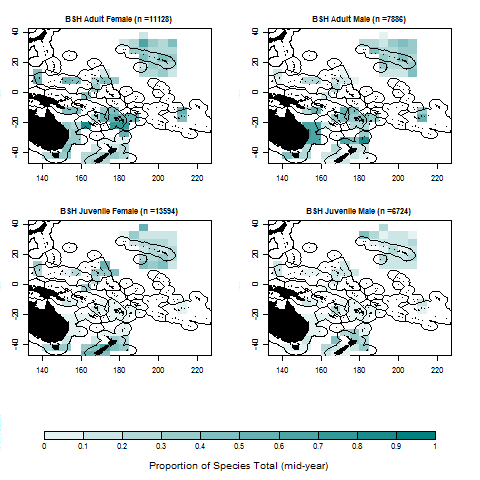
\includegraphics[width=\textwidth]{../GRAPHICS/Defined/BI_20_Map_maturity_sex_BSH_MY}
       \caption{Mid-year estimates.}
       \label{fig:test1}
   \end{subfigure}
   \begin{subfigure}[b]{0.6\textwidth}
       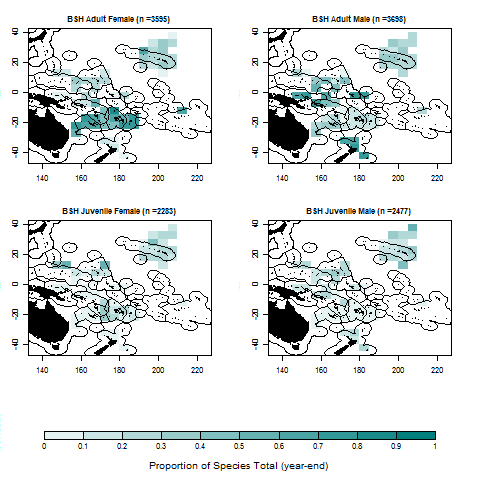
\includegraphics[width=\textwidth]{../GRAPHICS/Defined/BI_19_Map_maturity_sex_BSH}
       \caption{End of year estimates.}
       \label{fig:test2}
   \end{subfigure}
\caption{Blue Shark:  Proportion observed in each 5 x 5 degree cell which were adult females, adult males, juvenile females and juvenile males for mid-year (left panel) and year-end (right panel) periods. Darker cell shading indicates higher proportions observed. Samples sizes shown are those before removing cells with less than 20 individuals from the analysis. }
\label{fig:test} 
\end{figure}
\end{landscape}


%% Silky
\begin{landscape}
\begin{figure}
\centering
   \begin{subfigure}[b]{0.6\textwidth}
       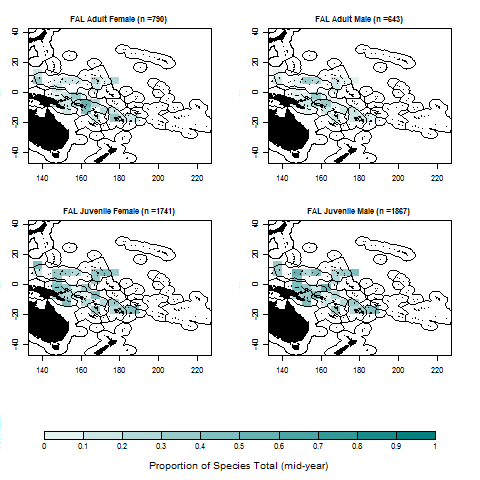
\includegraphics[width=\textwidth]{../GRAPHICS/Defined/BI_22_Map_maturity_sex_FAL_MY}
       \caption{Mid-year estimates.}
       \label{fig:test1}
   \end{subfigure}
   \begin{subfigure}[b]{0.6\textwidth}
       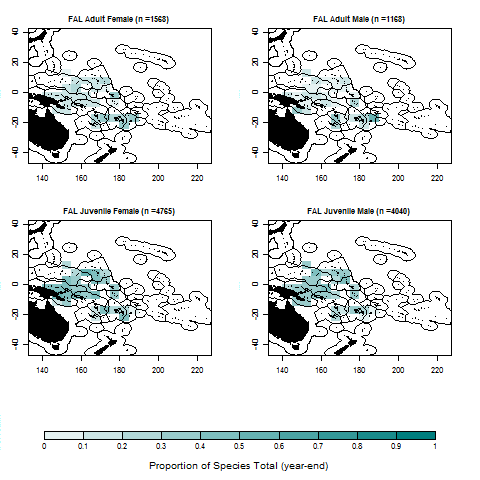
\includegraphics[width=\textwidth]{../GRAPHICS/Defined/BI_21_Map_maturity_sex_FAL}
       \caption{End of year estimates.}
       \label{fig:test2}
   \end{subfigure}
\caption{Silky Shark: Proportion observed in each 5 x 5 degree cell which were adult females, adult males, juvenile females and juvenile males for mid-year (left panel) and year-end (right panel) periods. Darker cell shading indicates higher proportions observed. Samples sizes shown are those before removing cells with less than 20 individuals from the analysis. }
\label{fig:test} 
\end{figure}
\end{landscape}

%% Hammerhead
\begin{landscape}
\begin{figure}
\centering
   \begin{subfigure}[b]{0.6\textwidth}
       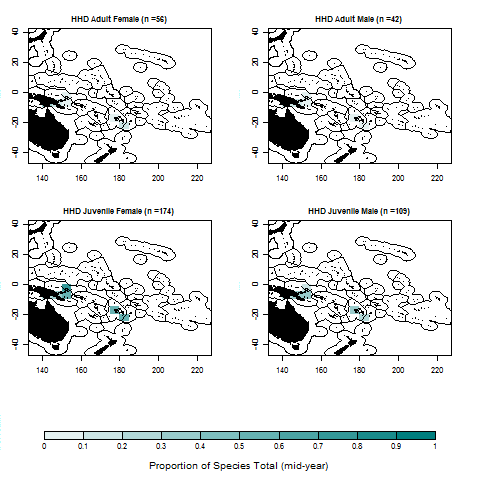
\includegraphics[width=\textwidth]{../GRAPHICS/Defined/BI_24_Map_maturity_sex_HHD_MY}
       \caption{Mid-year estimates.}
       \label{fig:test1}
   \end{subfigure}
   \begin{subfigure}[b]{0.6\textwidth}
       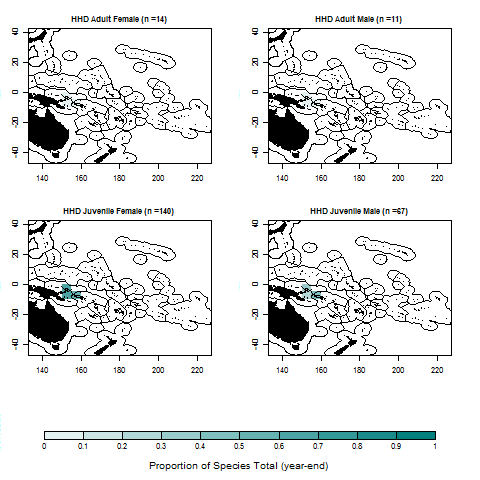
\includegraphics[width=\textwidth]{../GRAPHICS/Defined/BI_23_Map_maturity_sex_HHD}
       \caption{End of year estimates.}
       \label{fig:test2}
   \end{subfigure}
\caption{Hammerhead Shark: Proportion observed in each 5 x 5 degree cell which were adult females, adult males, juvenile females and juvenile males for mid-year (left panel) and year-end (right panel) periods. Darker cell shading indicates higher proportions observed. Samples sizes shown are those before removing cells with less than 20 individuals from the analysis. }
\label{fig:test} 
\end{figure}
\end{landscape}

%% Mako
\begin{landscape}
\begin{figure}
\centering
   \begin{subfigure}[b]{0.6\textwidth}
       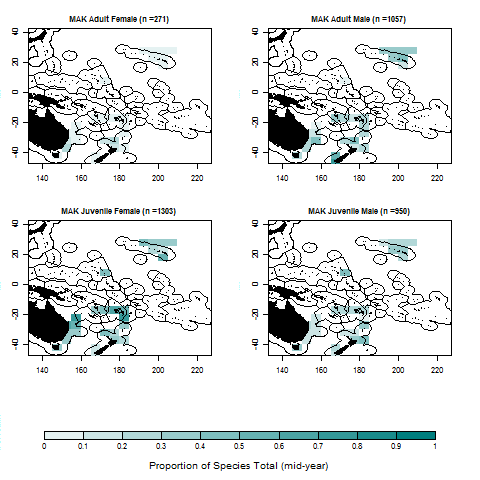
\includegraphics[width=\textwidth]{../GRAPHICS/Defined/BI_26_Map_maturity_sex_MAK_MY}
       \caption{Mid-year estimates.}
       \label{fig:test1}
   \end{subfigure}
   \begin{subfigure}[b]{0.6\textwidth}
       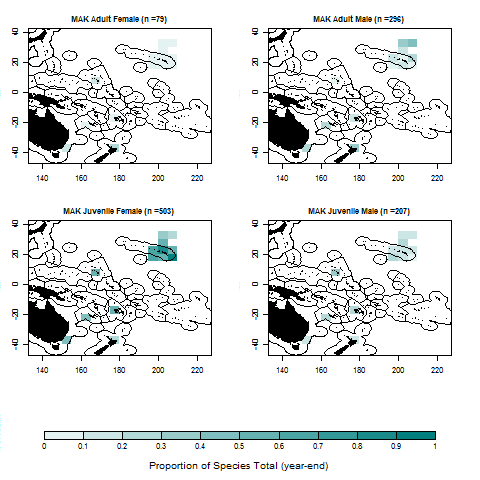
\includegraphics[width=\textwidth]{../GRAPHICS/Defined/BI_25_Map_maturity_sex_MAK}
       \caption{End of year estimates.}
       \label{fig:test2}
   \end{subfigure}
\caption{Mako Shark: Proportion observed in each 5 x 5 degree cell which were adult females, adult males, juvenile females and juvenile males for mid-year (left panel) and year-end (right panel) periods. Darker cell shading indicates higher proportions observed. Samples sizes shown are those before removing cells with less than 20 individuals from the analysis. }
\label{fig:test} 
\end{figure}
\end{landscape}

%% OCS
\begin{landscape}
\begin{figure}
\centering
   \begin{subfigure}[b]{0.6\textwidth}
       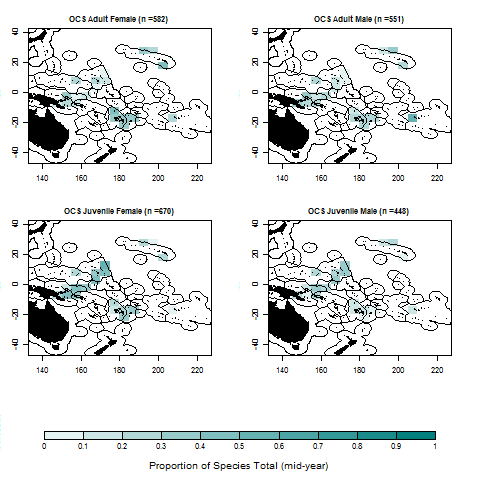
\includegraphics[width=\textwidth]{../GRAPHICS/Defined/BI_28_Map_maturity_sex_OCS_MY}
       \caption{Mid-year estimates.}
       \label{fig:test1}
   \end{subfigure}
   \begin{subfigure}[b]{0.6\textwidth}
       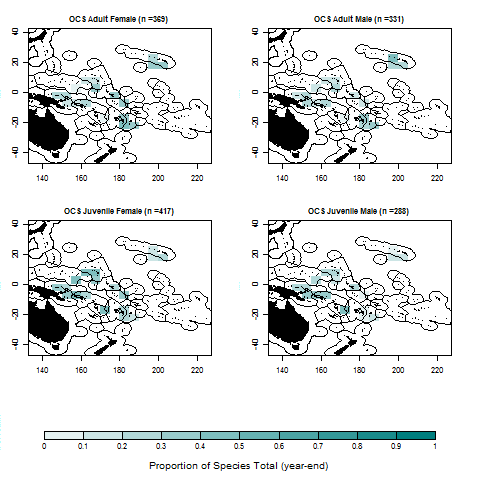
\includegraphics[width=\textwidth]{../GRAPHICS/Defined/BI_27_Map_maturity_sex_OCS}
       \caption{End of year estimates.}
       \label{fig:test2}
   \end{subfigure}
\caption{Oceanic Whitetip Shark: Proportion observed in each 5 x 5 degree cell which were adult females, adult males, juvenile females and juvenile males for mid-year (left panel) and year-end (right panel) periods. Darker cell shading indicates higher proportions observed. Samples sizes shown are those before removing cells with less than 20 individuals from the analysis. }
\label{fig:test} 
\end{figure}
\end{landscape}

%% Porbeagle
\begin{landscape}
\begin{figure}
\centering
   \begin{subfigure}[b]{0.6\textwidth}
       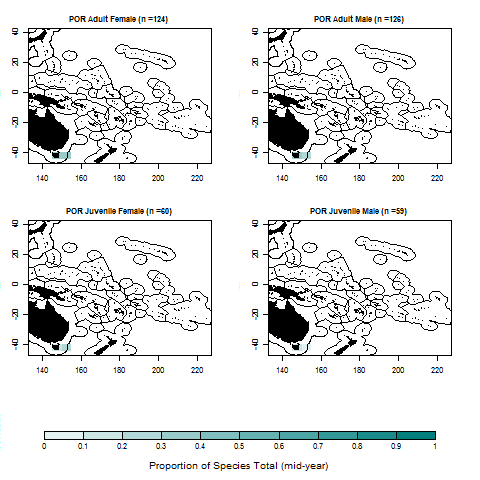
\includegraphics[width=\textwidth]{../GRAPHICS/Defined/BI_30_Map_maturity_sex_POR_MY}
       \caption{Mid-year estimates.}
       \label{fig:test1}
   \end{subfigure}
   \begin{subfigure}[b]{0.6\textwidth}
       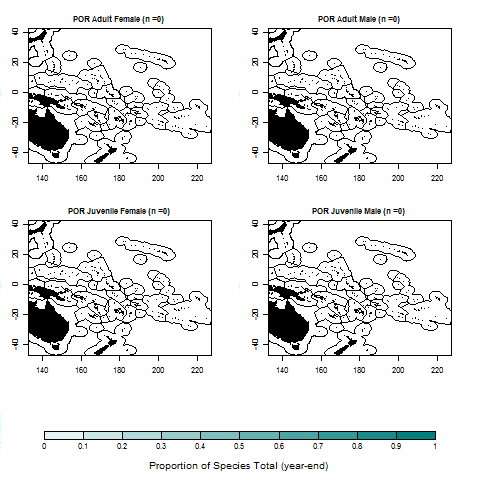
\includegraphics[width=\textwidth]{../GRAPHICS/Defined/BI_29_Map_maturity_sex_POR}
       \caption{End of year estimates.}
       \label{fig:test2}
   \end{subfigure}
\caption{Porbeagle Shark: Proportion observed in each 5 x 5 degree cell which were adult females, adult males, juvenile females and juvenile males for mid-year (left panel) and year-end (right panel) periods. Darker cell shading indicates higher proportions observed. Samples sizes shown are those before removing cells with less than 20 individuals from the analysis. }
\label{fig:test} 
\end{figure}
\end{landscape}

%% Thresher
\begin{landscape}
\begin{figure}
\centering
   \begin{subfigure}[b]{0.6\textwidth}
       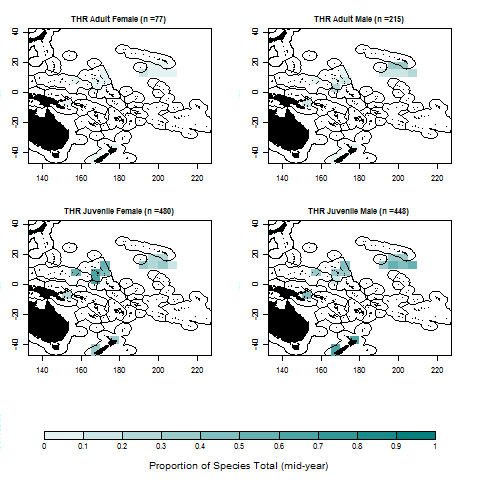
\includegraphics[width=\textwidth]{../GRAPHICS/Defined/BI_32_Map_maturity_sex_THR_MY}
       \caption{Mid-year estimates.}
       \label{fig:test1}
   \end{subfigure}
   \begin{subfigure}[b]{0.6\textwidth}
       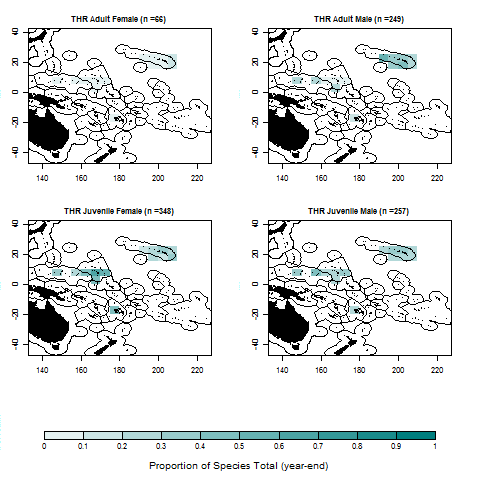
\includegraphics[width=\textwidth]{../GRAPHICS/Defined/BI_31_Map_maturity_sex_THR}
       \caption{End of year estimates.}
       \label{fig:test2}
   \end{subfigure}
\caption{Thresher Shark: Proportion observed in each 5 x 5 degree cell which were adult females, adult males, juvenile females and juvenile males for mid-year (left panel) and year-end (right panel) periods. Darker cell shading indicates higher proportions observed. Samples sizes shown are those before removing cells with less than 20 individuals from the analysis. }
\label{fig:test} 
\end{figure}
\end{landscape}


%% UPPER JAW FORK LENGTH
\addcenterfigLS[Sex ratio (proportion female) of shark species caught by longline gear in the WCPO. The number of samples available for each sex and region is also shown.]{fig:map}{../GRAPHICS/Defined/BI_01_LLSexRatio_RDS}

\addcenterfig[Blue shark: median upper jaw fork length by year and region for males and females. Solid line shows median values, greyed area shows the limits of the 5th and 95th percentiles. The number of samples available for each sex and region is also shown.]{fig:map}{../GRAPHICS/Defined/BI_02_bio_len_BSH_RDS}

\addcenterfig[Silky shark: median upper jaw fork length by year and region for males and females. Solid line shows median values, greyed area shows the limits of the 5th and 95th percentiles. The number of samples available for each sex and region is also shown.]{fig:map}{../GRAPHICS/Defined/BI_03_bio_len_FAL_RDS}

\addcenterfig[Hammerhead shark: median upper jaw fork length by year and region for males and females. Solid line shows median values, greyed area shows the limits of the 5th and 95th percentiles. The number of samples available for each sex and region is also shown.]{fig:map}{../GRAPHICS/Defined/BI_04_bio_len_HHD_RDS}

\addcenterfig[Mako shark: median upper jaw fork length by year and region for males and females. Solid line shows median values, greyed area shows the limits of the 5th and 95th percentiles. The number of samples available for each sex and region is also shown.]{fig:map}{../GRAPHICS/Defined/BI_05_bio_len_MAK_RDS}

\addcenterfig[Oceanic Whitetip shark: median upper jaw fork length by year and region for males and females. Solid line shows median values, greyed area shows the limits of the 5th and 95th percentiles. The number of samples available for each sex and region is also shown.]{fig:map}{../GRAPHICS/Defined/BI_06_bio_len_OCS_RDS}

\addcenterfig[Porbeagle shark: median upper jaw fork length by year and region for males and females. Solid line shows median values, greyed area shows the limits of the 5th and 95th percentiles. The number of samples available for each sex and region is also shown.]{fig:map}{../GRAPHICS/Defined/BI_07_bio_len_POR_RDS}

\addcenterfig[Thresher shark: median upper jaw fork length by year and region for males and females. Solid line shows median values, greyed area shows the limits of the 5th and 95th percentiles. The number of samples available for each sex and region is also shown.]{fig:map}{../GRAPHICS/Defined/BI_08_bio_len_THR_RDS}


\addcenterfig[Silky shark: median upper jaw fork length by year and region for both sexes combined, observed in the   purse seine fishery. Solid black line shows median values, dashed lines show the limits of the 5th and 95th percentiles. The number of samples available for each sex and region is also shown.]{fig:map}{../GRAPHICS/Defined/BI_09_ps_bio_len_FAL}

\addcenterfig[Oceanic whitetip shark: median upper jaw fork length by year and region for both sexes combined, observed in the   purse seine fishery. Solid black line shows median values, dashed lines show the limits of the 5th and 95th percentiles. The number of samples available for each sex and region is also shown.]{fig:map}{../GRAPHICS/Defined/BI_10_ps_bio_len_OCS}


\clearpage


\addcenterfig[Blue shark: standardised length for male and females for longline data. Light grey line shows a lowess smoother.]{fig:map}{../GRAPHICS/Defined/BI_11_len_stdz_Blue_RDS}

\addcenterfig[Silky shark: standardised length for male and females for longline data. Light grey line shows a lowess smoother.]{fig:map}{../GRAPHICS/Defined/BI_12_len_stdz_Silky_RDS}

\addcenterfig[Hammerhead shark: standardised length for male and females for longline data. Light grey line shows a lowess smoother.]{fig:map}{../GRAPHICS/Defined/BI_13_len_stdz_Hammerhead_RDS}

\addcenterfig[Mako shark: standardised length for male and females. Light grey line shows a lowess smoother.]{fig:map}{../GRAPHICS/Defined/BI_14_len_stdz_Mako_RDS}

\addcenterfig[Oceanic Whitetip shark: standardised length for male and females for longline data. Light grey line shows a lowess smoother.]{fig:map}{../GRAPHICS/Defined/BI_15_len_stdz_OceanicWhiteTip}

\addcenterfig[Porbeagle shark: standardised length for male and females for longline data. Light grey line shows a lowess smoother.]{fig:map}{../GRAPHICS/Defined/BI_16_len_stdz_Porbeagle_RDS}

\addcenterfig[Thresher shark: standardised length for male and females for longline data. Light grey line shows a lowess smoother.]{fig:map}{../GRAPHICS/Defined/BI_17_len_stdz_Thresher_RDS}

\addcenterfig[Annual change in length (cm) over the study period as derived from the year effect of a GLM fitted to the sex and species specific data shown in figures 71 to 77 ]{fig:map}{../GRAPHICS/Defined/BI_18_len_stdz_coef_out}
%%%%%%%%%%%%%%%%%%%%%%%%%%%%%%%%%%%%%%%%%%%%%%%%%%%%%%%%%%%%%%%%%%%%%%%%%%%%%%%%%%%%%%%%%%%%%%%%%%%%%%%%%%%%%%%%%%%%%%%%%%
\clearpage
\section{Whale Shark Figures}
\addcenterfig[Annual number of observed free school sets (bars) and proportion of sets with some form of whale shark interaction (see text for criteria).]{fig:whaleshark1}{../GRAPHICS/Whale-Shark-Picture-1}

\addcenterfig[Contour plots based on 1 $\times$ 1 degree square data for all years combined of purse seine sets (top), whale shark records (middle – see text for criteria), and encounter rates (bottom --- simply whale shark records divided by total sets for each 1 x1 degree square). Grey represents zeros, white are NA’s (e.g. zero whale sharks divided by zero sets), and the scale increases from green to yellow to orange to pink to red.]{fig:whaleshark2}{../GRAPHICS/Whale-Shark-Picture-2}
%%%%%%%%%%%%%%%%%%%%%%%%%%%%%%%%%%%%%%%%%%%%%%%%%%%%%%%%%%%%%%%%%%%%%%%%%%%%%%%%%%%%%%%%%%%%%%%%%%%%%%%%%%%%%%%%%%%%%%%%%%
\clearpage
\section{Management Considerations}

\addcenterfig[Fate of observed sharks caught by longline in the WCPO (total numbers for all species combined).]{fig:map}{../GRAPHICS/fate_ll_obs_by_region}

\addcenterfig[Fate of observed sharks caught by longline in the WCPO (proportion by number for all species combined).]{fig:map}{../GRAPHICS/fate_ll_ps_obs_all_keysharks_wcpo}


\addcenterfig[Fate of observed blue sharks caught by longline in the WCPO.]{fig:map}{../GRAPHICS/fate_ll_obs_BSH}
\addcenterfig[Fate of observed silky sharks caught by longline in the WCPO.]{fig:map}{../GRAPHICS/fate_ll_obs_FAL}
\addcenterfig[Fate of observed hammerhead sharks caught by longline in the WCPO.]{fig:map}{../GRAPHICS/fate_ll_obs_HHD}
\addcenterfig[Fate of observed mako sharks caught by longline in the WCPO.]{fig:map}{../GRAPHICS/fate_ll_obs_MAK}
\addcenterfig[Fate of observed oceanic whitetip sharks caught by longline in the WCPO.]{fig:map}{../GRAPHICS/fate_ll_obs_OCS}
\addcenterfig[Fate of observed porbeagle sharks caught by longline in the WCPO.]{fig:map}{../GRAPHICS/fate_ll_obs_POR}
\addcenterfig[Fate of observed thresher sharks caught by longline in the WCPO.]{fig:map}{../GRAPHICS/fate_ll_obs_THR}


\section{Model Diagnostics}
\subsubsection{CPUE Standardisation Diagnostics}

\addcenterfig[[CPUE indicators, model diagnostics for blue shark (north) CPUE standardization via negative binomial model.]{fig:diagnobluen}{../GRAPHICS/BSH.north_MU~yy+program_code + HPBCAT2 + mm + sharkbait_SIGMA~program_code + HPBCAT2 + mm_resids}

\addcenterfig[CPUE indicators, model diagnostics for blue shark (north) CPUE standardization via negative binomial model.]{fig:map}{../GRAPHICS/SHK-GLM-vars-bp-smry_BSH.north}


\addcenterfig[CPUE indicators, model diagnostics for blue shark (south) CPUE standardization via negative binomial model.]{fig:map}{../GRAPHICS/BSH.south_MU~yy+flag + HPBCAT2 + mm + sharkbait_SIGMA~intrcpt_resids}

\addcenterfig[CPUE indicators, model diagnostics for blue shark (south) CPUE standardization via negative binomial model.]{fig:map}{../GRAPHICS/SHK-GLM-vars-bp-smry_BSH.south}


\addcenterfig[CPUE indicators, model diagnostics for silky shark CPUE standardization via negative binomial model.]{fig:map}{../GRAPHICS/FAL_MU~yy+program_code + HPBCAT2 + mm + sharkbait_SIGMA~program_code + sharkbait + mm_resids}

\addcenterfig[CPUE indicators, model diagnostics for silky shark CPUE standardization via negative binomial model.]{fig:map}{../GRAPHICS/SHK-GLM-vars-bp-smry_FAL}

\clearpage
\addcenterfig[CPUE indicators, model diagnostics for hammerhead shark CPUE standardization via negative binomial model]{fig:map}{../GRAPHICS/HHD_MU~yy+program_code + HPBCAT2 + mm + sharkbait_SIGMA~sharkbait_resids}

\addcenterfig[CPUE indicators, model diagnostics for hammerhead shark CPUE standardization via negative binomial model]{fig:map}{../GRAPHICS/SHK-GLM-vars-bp-smry_HHD}


\addcenterfig[CPUE indicators, model diagnostics for mako shark (northern hemisphere) CPUE standardization via negative binomial model.]{fig:map}{../GRAPHICS/MAK.north_MU~yy+program_code + mm + sharkbait_SIGMA~HPBCAT2_resids}

\addcenterfig[CPUE indicators, model diagnostics for mako shark (northern hemisphere) CPUE standardization via negative binomial model.]{fig:map}{../GRAPHICS/SHK-GLM-vars-bp-smry_MAK.north}


\addcenterfig[CPUE indicators, model diagnostics for mako shark (southern hemisphere) CPUE standardization via negative binomial model.]{fig:map}{../GRAPHICS/MAK.south_MU~yy+program_code + HPBCAT2 + mm + sharkbait_SIGMA~program_code + mm_resids}

\addcenterfig[CPUE indicators, model diagnostics for mako shark (southern hemisphere) CPUE standardization via negative binomial model.]{fig:map}{../GRAPHICS/SHK-GLM-vars-bp-smry_MAK.south}


\addcenterfig[CPUE indicators, model diagnostics for oceanic whitetip shark CPUE standardization via negative binomial model.]{fig:map}{../GRAPHICS/OCS_MU~yy+program_code + HPBCAT2 + mm + sharkbait_SIGMA~program_code_resids}

\addcenterfig[CPUE indicators, model diagnostics for oceanic whitetip shark CPUE standardization via negative binomial model.]{fig:map}{../GRAPHICS/SHK-GLM-vars-bp-smry_OCS}

\addcenterfig[CPUE indicators, model diagnostics for porbeagle shark CPUE standardization via negative binomial model.]{fig:map}{../GRAPHICS/POR_MU~yy + flag + HPBCAT2 + mm_SIGMA~flag + mm_resids}

\addcenterfig[CPUE indicators, model diagnostics for porbeagle shark CPUE standardization via negative binomial model.]{fig:map}{../GRAPHICS/SHK-GLM-vars-bp-smry_POR}


\addcenterfig[[CPUE indicators, model diagnostics for silky thresher CPUE standardization via negative binomial model.]{fig:diagnosilky}{../GRAPHICS/THR_MU~yy+program_code + HPBCAT2 + mm_SIGMA~HPBCAT2 + program_code_resids}

\addcenterfig[CPUE indicators, model diagnostics for thresher CPUE standardization via negative binomial model.]{fig:map}{../GRAPHICS/SHK-GLM-vars-bp-smry_THR}

\clearpage
\BSHnorthaic
\BSHsouthaic
\FALaic
\HHDaic
\MAKnorthaic
\MAKsouthaic
\OCSaic
\PORaic
\THRaic